% 3 种交叉 + 4 种变异：编码条形示意图
% 排版：说明文字与基因条分行（文字在上，条形在下），减少遮挡
% 编译：xelatex AMO_operator_encoding_diagrams_tikz.tex
\documentclass[a4paper,10pt]{article}
\usepackage[margin=11mm]{geometry}
\usepackage{ctex}
\usepackage{tikz}
\usetikzlibrary{calc,positioning,fit,backgrounds}
\usepackage{graphicx}

\newlength{\AMOHalf}
\setlength{\AMOHalf}{0.48\linewidth}

\newlength{\genestep}
\setlength{\genestep}{6.15mm}

\tikzset{
  gene/.style={
    draw=black,
    line width=0.55pt,
    minimum width=6.2mm,
    minimum height=6.4mm,
    inner sep=0pt,
    font=\footnotesize\bfseries,
    align=center
  },
  lbl/.style={font=\footnotesize, inner sep=0pt, anchor=north west},
  ttl/.style={font=\bfseries\footnotesize, inner sep=0pt, anchor=north west},
  panelframe/.style={draw=gray!55, rounded corners=2pt, inner sep=8pt, fill=white, fill opacity=0.96},
}

% #1=节点名前缀 #2=yshift #3=基因/颜色列表 → 生成 #11,#12,...,#19
\newcommand{\GeneRowPref}[3]{%
  \begin{scope}[yshift=#2]
    \foreach \g/\c [count=\i] in {#3} {
      \node[gene, fill=\c] (#1\i) at ({(\i-1)*\genestep},0) {\g};
    }
  \end{scope}
}

\begin{document}
\begin{center}
{\large\bfseries AMO 编码示意图（交叉 $\times$3 + 变异 $\times$4）}\\[1mm]
{\footnotesize 约定：\texttt{1..4} 商家；\texttt{5..8} 客户（客户=商家$+4$）；\texttt{0} 为段间分隔符（$m{=}2$ 时 1 个 \texttt{0}）。}
\end{center}

\vspace{2mm}
\noindent\textbf{图例（按对配色）：}\ 
{\footnotesize 蓝\texttt{1-5}；绿\texttt{2-6}；橙\texttt{3-7}；粉紫\texttt{4-8}；灰\texttt{0}。}

\vspace{2mm}
\noindent
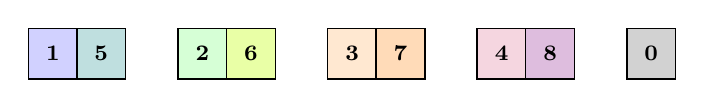
\begin{tikzpicture}[baseline=(L1.base)]
  \GeneRowPref{L}{0mm}{1/blue!18,5/teal!25}
  \begin{scope}[xshift=19mm]
    \GeneRowPref{M}{0mm}{2/green!16,6/lime!35}
  \end{scope}
  \begin{scope}[xshift=38mm]
    \GeneRowPref{N}{0mm}{3/orange!18,7/orange!28}
  \end{scope}
  \begin{scope}[xshift=57mm]
    \GeneRowPref{O}{0mm}{4/purple!16,8/violet!26}
  \end{scope}
  \begin{scope}[xshift=76mm]
    \GeneRowPref{Z}{0mm}{0/gray!35}
  \end{scope}
\end{tikzpicture}

\vspace{5mm}

% ===================== 第 1 页：三个交叉 =====================
\noindent\begin{tikzpicture}
  \begin{scope}[local bounding box=BXp1]
    \node[ttl] (PTtit) at (0,0) {(1) 交叉：PTC（位置追踪）};
    \node[lbl, below=3mm of PTtit.south west] (PTl1) {父代1 $P_1$：};
    \node[lbl, below=1.5mm of PTl1.south west, align=left, font=\scriptsize] (PTcut)
      {切点 $k$（安全位置）：竖虚线标于下方基因条。};
    \begin{scope}[shift={($(PTcut.south west)+(0,-2mm)$)}]
      \GeneRowPref{PA}{0mm}{1/blue!18,5/blue!18,2/blue!18,6/blue!18,0/gray!35,3/blue!18,7/blue!18,4/blue!18,8/blue!18}
      \draw[dashed, line width=0.85pt] ($(PA4.east)+(0.75mm,3.4mm)$) -- ($(PA4.east)+(0.75mm,-3.4mm)$);
    \end{scope}
    \node[lbl, below=4mm of PA9.south west] (PTl2) {父代2 $P_2$：};
    \begin{scope}[shift={($(PTl2.south west)+(0,-2mm)$)}]
      \GeneRowPref{PB}{0mm}{2/green!16,6/green!16,1/green!16,5/green!16,0/gray!35,4/green!16,8/green!16,3/green!16,7/green!16}
    \end{scope}
    \node[lbl, below=4mm of PB9.south west, text width=0.92\linewidth, align=left] (PTl3)
      {子代（示意）：左半段复制 $P_1$；右半段按 $P_2$ 从左到右扫描填充，客户仅在其商家已出现后加入。};
    \begin{scope}[shift={($(PTl3.south west)+(0,-2mm)$)}]
      \GeneRowPref{PC}{0mm}{1/blue!18,5/blue!18,2/blue!18,6/blue!18,0/gray!35,4/green!16,8/green!16,3/green!16,7/green!16}
    \end{scope}
  \end{scope}
  \scoped[on background layer]{\node[panelframe, fit=(BXp1), inner sep=7pt] {};}
\end{tikzpicture}\par

\vspace{5mm}

\noindent\resizebox{\linewidth}{!}{%
\begin{tikzpicture}
  \begin{scope}[local bounding box=BXp2]
    \node[ttl] (PCtit) at (0,0) {(2) 交叉：PPC（对优先级）};
    \node[lbl, below=2mm of PCtit.south west, text width=0.96\linewidth, align=left] (PCdesc)
      {\scriptsize 商家 $s$ 的优先级取两父代首次出现位置的较小者；按优先级排列商家，并向右用首个 \texttt{0} 槽插入对应客户（实现细节见源码）。};
    \node[lbl, below=3mm of PCdesc.south west] (PCl1) {父代 $P_1$：};
    \begin{scope}[shift={($(PCl1.south west)+(0,-2mm)$)}]
      \GeneRowPref{QA}{0mm}{1/blue!18,5/blue!18,2/blue!18,6/blue!18,0/gray!35,3/blue!18,7/blue!18,4/blue!18,8/blue!18}
    \end{scope}
    \node[lbl, below=4mm of QA9.south west] (PCl2) {父代 $P_2$：};
    \begin{scope}[shift={($(PCl2.south west)+(0,-2mm)$)}]
      \GeneRowPref{QB}{0mm}{2/green!16,6/green!16,1/green!16,5/green!16,0/gray!35,4/green!16,8/green!16,3/green!16,7/green!16}
    \end{scope}
    \node[lbl, below=4mm of QB9.south west] (PCl3) {子代（示例，按对配色）：};
    \begin{scope}[shift={($(PCl3.south west)+(0,-2mm)$)}]
      \GeneRowPref{QC}{0mm}{2/green!16,1/blue!18,4/purple!16,3/orange!18,0/gray!35,6/lime!35,5/teal!25,8/violet!26,7/orange!28}
    \end{scope}
  \end{scope}
  \scoped[on background layer]{\node[panelframe, fit=(BXp2), inner sep=7pt] {};}
\end{tikzpicture}%
}\par

\vspace{5mm}

\noindent\resizebox{\linewidth}{!}{%
\begin{tikzpicture}
  \begin{scope}[local bounding box=BXp3]
    \node[ttl] (POtit) at (0,0) {(3) 交叉：OPC（顺序保持）};
    \node[lbl, below=2mm of POtit.south west, text width=0.96\linewidth, align=left] (POdesc)
      {\scriptsize 抽取两父代商家遍历顺序，随机切点融合并补全商家；其后构造与 PPC 类似。示例：$O_1{=}[1,2,3,4]$，$O_2{=}[2,1,4,3]$，$f{=}2 \Rightarrow F{=}[1,2,4,3]$。};
    \node[lbl, below=3mm of POdesc.south west] (POl1) {子代（示例）：};
    \begin{scope}[shift={($(POl1.south west)+(0,-2mm)$)}]
      \GeneRowPref{RA}{0mm}{1/blue!18,2/green!16,4/purple!16,3/orange!18,0/gray!35,5/teal!25,6/lime!35,8/violet!26,7/orange!28}
    \end{scope}
  \end{scope}
  \scoped[on background layer]{\node[panelframe, fit=(BXp3), inner sep=7pt] {};}
\end{tikzpicture}%
}\par

\clearpage

% ===================== 第 2 页：四个变异 =====================
\noindent\begin{tikzpicture}
  \begin{scope}[local bounding box=BXt12]
    \begin{scope}[local bounding box=BXt1]
      \node[ttl] (T1t) at (0,0) {(4) 变异 T1：商家 $\rightarrow$ 段首};
      \node[lbl, below=2mm of T1t.south west] (T1la) {操作前：};
      \begin{scope}[shift={($(T1la.south west)+(0,-2mm)$)}]
        \GeneRowPref{S1}{0mm}{1/blue!18,5/blue!18,2/blue!18,6/blue!18,0/gray!35,3/blue!18,7/blue!18,4/blue!18,8/blue!18}
      \end{scope}
      \node[lbl, below=4mm of S19.south west] (T1lb) {操作后：};
      \begin{scope}[shift={($(T1lb.south west)+(0,-2mm)$)}]
        \GeneRowPref{S2}{0mm}{1/blue!18,5/blue!18,2/blue!18,6/blue!18,0/gray!35,4/purple!16,3/blue!18,7/blue!18,8/blue!18}
      \end{scope}
    \end{scope}
    \begin{scope}[xshift=\AMOHalf, local bounding box=BXt2]
      \node[ttl] (T2t) at (0,0) {(5) 变异 T2：客户 $\rightarrow$ 段尾};
      \node[lbl, below=2mm of T2t.south west] (T2la) {操作前：};
      \begin{scope}[shift={($(T2la.south west)+(0,-2mm)$)}]
        \GeneRowPref{U1}{0mm}{1/blue!18,5/blue!18,2/blue!18,6/blue!18,0/gray!35,3/blue!18,7/blue!18,4/blue!18,8/blue!18}
      \end{scope}
      \node[lbl, below=4mm of U19.south west] (T2lb) {操作后：};
      \begin{scope}[shift={($(T2lb.south west)+(0,-2mm)$)}]
        \GeneRowPref{U2}{0mm}{1/blue!18,5/blue!18,2/blue!18,6/blue!18,0/gray!35,3/blue!18,4/blue!18,8/blue!18,7/orange!28}
      \end{scope}
    \end{scope}
  \end{scope}
  \scoped[on background layer]{\node[panelframe, fit=(BXt12), inner sep=7pt] {};}
\end{tikzpicture}\par

\vspace{6mm}

\noindent\begin{tikzpicture}
  \begin{scope}[local bounding box=BXt3]
    \node[ttl] (T3t) at (0,0) {(6) 变异 T3：滑动分隔符 \texttt{0}（仅在成对安全边界；示意）};
    \node[lbl, below=2mm of T3t.south west] (T3la) {操作前：};
    \begin{scope}[shift={($(T3la.south west)+(0,-2mm)$)}]
      \GeneRowPref{V1}{0mm}{1/blue!18,5/blue!18,2/blue!18,6/blue!18,0/gray!35,3/blue!18,7/blue!18,4/blue!18,8/blue!18}
    \end{scope}
    \node[lbl, below=4mm of V19.south west] (T3lb) {操作后：};
    \begin{scope}[shift={($(T3lb.south west)+(0,-2mm)$)}]
      \GeneRowPref{V2}{0mm}{1/blue!18,5/blue!18,2/blue!18,6/blue!18,3/blue!18,7/blue!18,0/gray!35,4/blue!18,8/blue!18}
    \end{scope}
  \end{scope}
  \scoped[on background layer]{\node[panelframe, fit=(BXt3), inner sep=7pt] {};}
\end{tikzpicture}\par

\vspace{6mm}

\noindent\begin{tikzpicture}
  \begin{scope}[local bounding box=BXt4]
    \node[ttl] (T4t) at (0,0) {(7) 变异 T4：跨段迁移整对（\texttt{4} 与 \texttt{8} 一起剪切--粘贴）};
    \node[lbl, below=2mm of T4t.south west] (T4la) {操作前：};
    \begin{scope}[shift={($(T4la.south west)+(0,-2mm)$)}]
      \GeneRowPref{W1}{0mm}{1/blue!18,5/blue!18,2/blue!18,6/blue!18,0/gray!35,3/blue!18,7/blue!18,4/purple!16,8/violet!26}
      \draw[->, line width=0.9pt, red!65!black] ($(W18.east)+(1.2mm,0)$)
        .. controls +(8mm,7mm) and +(-10mm,7mm) .. ($(W14.west)+(-10mm,2mm)$);
    \end{scope}
    \node[lbl, below=5mm of W19.south west] (T4lb) {操作后：};
    \begin{scope}[shift={($(T4lb.south west)+(0,-2mm)$)}]
      \GeneRowPref{W2}{0mm}{1/blue!18,5/blue!18,2/blue!18,6/blue!18,4/purple!16,8/violet!26,0/gray!35,3/blue!18,7/blue!18}
    \end{scope}
  \end{scope}
  \scoped[on background layer]{\node[panelframe, fit=(BXt4), inner sep=7pt] {};}
\end{tikzpicture}\par

\vspace{3mm}
\noindent{\footnotesize\textbf{提示：}全文为“先说明、后条形”的分行排版；若仍过宽，可把 \texttt{\textbackslash genestep} 略调小。}

\end{document}
